\documentclass[main]{subfiles}

\begin{document}


\chapter{Modelo F\'isico}
\label{chap:modelo}
Resulta imprescindible para controlar el cuadric\'optero comprender cabalmente su comportamiento. Con esta \'optica, lo que se busca es obtener el modelo m\'as sencillo que sea capaz de representar adecuadamente al sistema. El objetivo de este cap\'itulo es el de realizar el desarrollo de dicho modelo. La forma de modelar el sistema elegida es un Modelo en Variables de Estado, de ahora en m\'as MVE. Lo que se busca es obtener una representaci\'on del sistema de la forma $\dot{\vec{x}}=f\left(\vec{x},\vec{u},t\right)$, donde $\vec{x}$ es el vector de estados del sistema, $\vec{u}$ es el vector que representa las entradas del sistema y $t$ es el tiempo. \\

Al tratarse de una plataforma comercial no se dispone de todos los par\'ametros fundamentales para el desarrollo de dicho modelo, a modo de ejemplo, no se conoce como es la respuesta de los motores  ni el tensor de inercia del sistema (ver los cap\'itulos \ref{chap:test_motores} y \ref{chap:anexo_tensores} respectivamente). En el presente an\'alisis nos limitaremos a obtener las ecuaciones que gobiernan el comportamiento del cuadric\'optero.\\
    


\section{Hip\'otesis de trabajo}

No debe perderse de vista que el cuadric\'optero con el que se trabaja fue dise\~nado para ser comandado a trav\'es de un control remoto. Por dicho motivo es razonable que sus caracter\'isticas sean tales que le permitan a una persona volarlo desde el suelo. Parece perfectamente razonable que se haya dise\~nado el sistema para volar por tiempos limitados, distancias relativamente cortas y a bajas velocidades. Estas consideraciones permiten introducir diversas simplificaciones en el modelado.


\subsection{La Tierra como sistema de referencia inercial}
La Tierra {\bf no} es un sistema de referencia inercial ya que la misma se encuentra sometida a la traslaci\'on en torno al Sol y a una rotaci\'on en sobre su eje. Supongamos una part\'icula que se encuentra en movimiento relativo a la Tierra. Su aceleraci\'on respecto de un sistema verdaderamente inercial puede escribirse como:
\begin{equation}
\vec{a}=\vec{a\prime}+\vec{a_T} +\vec{a_C}
\end{equation}.

\begin{equation}
\vec{a_T}=\vec{a_{O\prime}}+\dot{\vec{\omega}}\times\vec{r\prime}+\vec{\omega}\times (\vec{\omega}\times\vec{r\prime})
\end{equation}

\begin{equation}
\vec{a_C}=2\vec{\omega}\times\vec{v\prime}
\end{equation}
En las ecuaciones anteriores $\vec{a\prime}$ es la aceleraci\'on de la part\'icula en el sistema relativo, $\vec{v\prime}$ es la velocidad relativa de la part\'icula, $\vec{r\prime}$ la posici\'on relativa, $\vec{\omega}$ es la velocidad angular de la Tierra y $\vec{a_{O\prime}}$ es la aceleraci\'on del centro de masa de la Tierra.

El objetivo es ahora analizar si es posible considerar que $\vec{a}\approx\vec{a\prime}$. Si esto \'ultimo se cumple se puede aproximar a la Tierra como un sistema inercial. El radio promedio de la \'orbita Helioc\'entrica($R_H$) es de $1.5\times10^8Km$, dicha \'orbita se recorre en 365 d\'ias lo que nos da una velocidad promedio de:

\begin{equation}
V_T=\frac{1.5\times10^{11}m}{365\times24\times60\times60s}\approx4.8\times10^3ms^{-1}
\end{equation}
Esta velocidad implica que la aceleraci\'on del centro de masa de la Tierra($\vec{a_{O\prime}}$) es de aproximadamente:

\begin{equation}
a_{O\prime}=\frac{V_T^2}{R_H}\approx15.36\times10^{-5}ms^{-2}
\end{equation}

Por otra parte sabemos que la Tierra rota sobre su eje una vez cada 24 horas con velocidad angular constante, tenemos as\'i que:

\begin{equation}
\omega=\frac{2\pi}{24\times60\times60s}\approx7.3\times10^{-5}rad s^{-1}
\end{equation}

Finalmente debemos considerar el radio promedio de la Tierra($R_T=6,731\times10^{6}m$), ya que las alturas que alcanzar\'a nuestro sistema son despreciables respecto del radio de la Tierra. 

Por lo tanto 
\begin{equation}
a_T \approx 3.6\times10^{-2}m^{s-2}
\end{equation}

Para que el t\'ermino de la aceleraci\'on de Coreolis sea comparable con la aceleraci\'on de transporte las velocidades del cuadric\'optero relativas a la Tierra deber\'ian ser del orden de cientos de metros por segundo, condici\'on que evidentemente no se cumple, por lo tanto este t\'ermino puede ser despreciado. 

La aceleraci\'on relativa al sistema de la Tierra difiere de  aproximadamente $3.6\times10^{-2}ms^{-2}$ de la aceleraci\'on medida en un sistema verdaderamente inercial. Por otra parte la resoluci\'on del aceler\'ometro utilizado es de $4mg\approx 4.81\times10^{-2}ms^{-2}$. Con el sensor elegido para trabajar es imposible distinguir entre ambas aceleraciones, por dicho motivo parece razonable despreciar el t\'ermino de la aceleraci\'on que corresponde a la aceleraci\'on de transporte. Esto nos permite afirmar que la Tierra puede aproximarse como un sistema de referencia inercial y por lo tanto se cumple que:

\begin{equation}
\sum \vec{F_{ext}}=m\vec{a}\approx m\vec{a\prime}
\end{equation}



\subsection{Curvatura de la Tierra}
El cuadric\'optero no se desplazara una distancia superior a una centena de metros paralelo a la superficie de la Tierra. Consideremos un caso extremo en el cual el cuadric\'optero se desplaza $1km$ en una direcci\'on. Esto corresponde a recorrer un arco de c\'irculo de $\theta = \frac{1km}{6,731\times10^{3}km}\approx 1.5\times 10^{-4}rad$. Si consideramos la superficie terrestre como un plano, la distancia recorrida es: 
\begin{equation}
d=R_T\sin(\theta) \approx 0.999999996km
\end{equation}

Como era de esperar, la diferencia entre la distancia recorrida como arco de c\'irculo y asumiendo una aproximaci\'on local de la Tierra por un plano es despreciable. Por lo tanto trabajaremos con un sistema de coordenadas cartesiano.
\subsection{Atracci\'on gravitacional}
Todos los objetos se encuentran relacionados entre s\'i por medio de la Fuerza de atracci\'on gravitacional. Sin embargo en las cercan\'ias de la Tierra la atracci\'on gravitacional con el resto de los objetos es completamente despreciable. Dicha fuerza vale:

\begin{equation}
F_G=G\frac{M_Tm}{d^2}=G\frac{M_Tm}{(R_T+h)^2} 
\end{equation}
Donde $G$ es la constante gravitacional y h la altura a la cual se encuentra una part\'icula.  
Como ya se analizo anteriormente las alturas a las cuales se desenvolver\'a el cuadric\'optero son despreciables respecto del radio de la Tierra. Por lo tanto la ecuaci\'on anterior queda:

\begin{equation}
F_G\approx\frac{M_Tm}{R_T^2}=gm
\end{equation}

donde g es la constante gravitacional de la Tierra, su valor es aproximadamente $9.81m^{s-2}$

\subsection{Fuerzas aerodin\'amicas}
Debido a las bajas velocidades que lograr\'a el cuadric\'optero se decidi\'o despreciar las fuerzas de tipo aerodin\'amicas, salvo aquellas responsables de las fuerzas y momentos de las h\'elices. Estas fuerzas ser\'an analizadas con mayor profundidad en la secci\'on \ref{FYT}.
\section{Sistema de referencia}

\begin{figure}
	\centering
	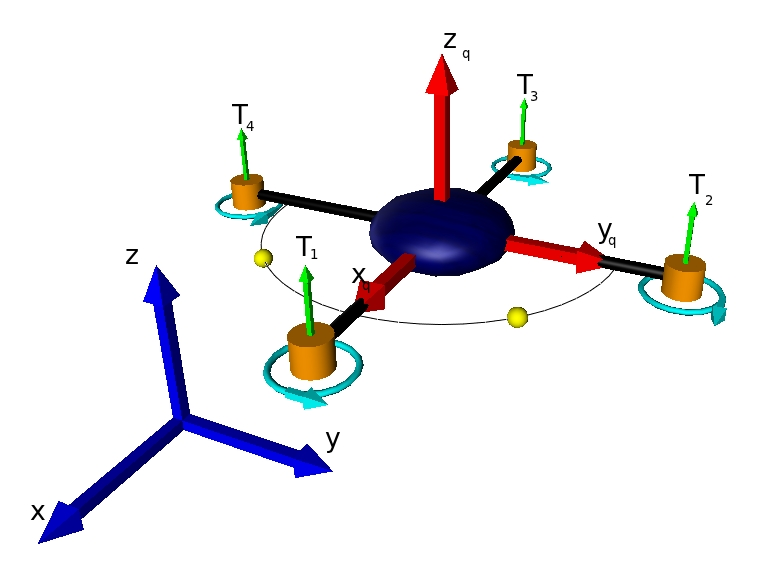
\includegraphics[width=0.7\textwidth]{./pics_modelo_fisico/quad_coord.jpg}
	\caption{Modelo del cuadc\'optero	}
	\label{fig:quad}
\end{figure}

A lo largo del presente desarrollo se trabajar\'a constantemente con dos sistemas de referencia: uno inercial solidario a la tierra ($S_I$) y otro solidario al cuadc\'optero ($S_q$) como se muestra en la figura \ref{fig:quad}. El sistema $S_I$ es un sistema local donde la direcci\'on $\vec{i}$, $\vec{j}$ y $\vec{k}$ corresponden a las direcciones Este, Norte y hacia arriba y el origen es la posici\'on inicial del cuadric\'optero. En la figura \ref{fig:quad} se pueden apreciar ambos sistemas de referencia.
El sistema $S_q$ se puede obtener realizando tres rotaciones compuestas del sistema $S_I$, dichas rotaciones se muestran en la figura \ref{fig:rotaciones}. Los \'angulos $\theta, \varphi$ y $\psi$ son conocidos como \'angulos de Euler.

\begin{figure} [h!]
  \centering
  \subfloat[Rotaci\'on seg\'un eje $\hat{k}$]{\label{fig:angulos_1}
  		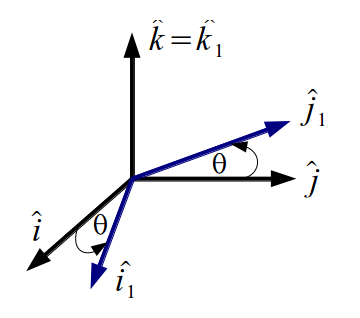
\includegraphics[width=0.3\textwidth]
  			{./pics_modelo_fisico/angulos_1.png}}
  \subfloat[Rotaci\'on seg\'un eje $\hat{j}$]{\label{fig:angulos_2} 
  		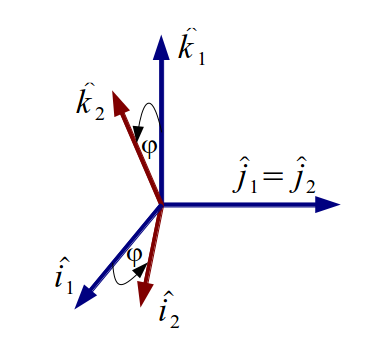
\includegraphics[width=0.3\textwidth]
  			{./pics_modelo_fisico/angulos_2.png}}
  \subfloat[Rotaci\'on seg\'un eje $\hat{i}$]{\label{fig:angulos_3} 
  		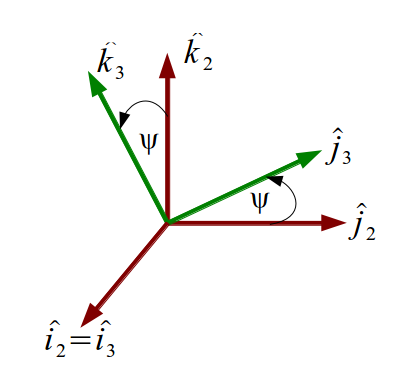
\includegraphics[width=0.3\textwidth]
  			{./pics_modelo_fisico/angulos_3.png}}
  \caption{Rotaciones}
  \label{fig:rotaciones}
\end{figure}

La importancia del sistema $S_q$ radica en las simplificaciones que introduce a la hora de escribir las ecuaciones, ya que por ejemplo en dicho sistema las direcciones del empuje de las h\'elices, de los torques que introducen y de las velocidades angulares de los motores del cuadric\'optero son constantes. Asimismo, algunos de los sensores del sistema de navegaci\'on (aceler\'ometro, gir\'oscopo y magnet\'ometro realizan medidas referenciadas al sistema de coordenadas solidario al cuadic\'optero, es decir en el sistema $S_q$. Considerar este sistema resulta en una simplificaci\'on del procesamiento de los datos obtenidos por la IMU. 

Las tres transformaciones pueden representarse matricialmente de la siguiente forma: 

\begin{equation}
\label{eq:bases}
H_I^1=\left(\begin{array}{ccc}
  \cos\theta&\sin\theta&0\\
  -\sin\theta&\cos\theta&0\\
  0&0&1\\
  \end{array}\right)   H_1^2=\left(\begin{array}{ccc}
  \cos\varphi&0& -\sin\varphi\\
  0&1&0\\
  \sin\varphi&0&\cos\varphi\\
  
  \end{array}\right)  H_2^q=\left(\begin{array}{ccc}
   1&0&0\\  
  0&\cos\psi&\sin\psi\\
  0&-\sin\psi&\cos\psi  
  
  \end{array}\right) 
\end{equation}



La transformaci\'on de las coordenadas del sistema inercial al sistema solidario al cuadric\'optero se obtiene realizando el producto de las tres matrices de rotaci\'on definidas.

\begin{footnotesize}
\begin{equation}
\label{eq:cambio_base}
H_I^q=H_2^q.H_1^2.H_I^1=\left(\begin{array}{ccc}
\cos\varphi\cos\theta& \cos\varphi\sin\theta& -\sin\varphi\\
 \cos\theta\sin\varphi\sin\psi -\cos\psi\sin\theta &\cos \psi \cos \theta+ \sin\varphi\sin\psi\sin\theta& \cos\varphi\sin\psi\\
\sin\psi\sin\theta + \cos\psi\cos\theta\sin\varphi&  \cos\psi\sin\varphi\sin\theta- \cos\theta\sin\psi & \cos\varphi\cos\psi\\
\end{array} \right)
\end{equation}
\end{footnotesize}
 
 A su vez, la transformaci\'on inversa puede obtenerse multiplicando las coordenadas del sistema $S_q$ por la matriz $H_q^I$. Dicha matriz puede obtenerse de la siguiente forma:
\begin{equation}
 H_q^I=(H_2^q.H_1^2.H_I^1)^{-1}=(H_I^1)^{-1}.(H_1^2)^{-1}.(H_2^q)^{-1}=H_1^I.H_2^1.H_q^2
 \end{equation}
 
\section{Cinem\'atica}
En primer lugar nos enfocaremos en comprender la relaci\'on que existe entre la velocidad angular del sistema y las derivadas de los \'angulos de Euler. Sea $\vec{\omega}$ la velocidad angular del cuadric\'optero (y por ende la del sistema $S_q$). La expresi\'on de la velocidad angular en el sistema de referencia del cuadric\'optero es la siguiente:
\begin{equation}
\vec{\omega}=w_{q_x}\vec{i_q}+w_{q_y}\vec{j_q}+w_{q_z}\vec{k_q}
\end{equation}
Donde $w_{q_x}$, $w_{q_y}$ y $w_{q_z}$ son las proyecciones ortogonales de la velocidad angular en el sistema $S_q$.
Por como fue construido el sistema de referencia solidario al cuadric\'optero y utilizando el teorema de adici\'on de velocidades angulares, se deduce trivialmente que la velocidad angular del cuadric\'optero puede escribirse como:

\begin{equation}
\vec{\omega}=\dot{\theta}\vec{k}+\dot{\varphi}\vec{j_1}+\dot{\psi}\vec{i_2}
\end{equation}

El vector $\vec{i_2}$ es invariante respecto de la tercer rotaci\'on, es decir que $\vec{i_2}=\vec{i_q}$. Por otra parte, multiplicando los vectores $\vec{k}$ y $\vec{j_1}$ por las matrices $H_1^2.H_2^q$ y $H_2^q$ respectivamente se puede obtener la velocidad angular del cuadric\'optero en el sistema de coordenadas referido a el. Operando se obtiene:

\begin{footnotesize}

\begin{equation}
w_{q_x}\vec{i_q}+w_{q_y}\vec{j_q}+w_{q_z}\vec{k_q}= (\dot{\psi}  +    \dot{\theta}\sin\varphi)\vec{i_q}+(\dot{\varphi}\cos\psi + \dot{\theta}\cos\varphi \sin\psi)\vec{j_q}+(\dot{\theta}\cos\varphi \cos\psi -  \dot{\varphi}\sin\psi)\vec{k_q}
\end{equation}
\end{footnotesize}

De esta ecuaci\'on se obtienen tres relaciones entre las velocidades angulares respecto de cada eje principal del sistema de coordenadas solidario al  cuadric\'optero con las derivadas de los \'angulos de Euler. Podemos re escribir dicha ecuaci\'on de la siguiente forma:

\begin{equation}
\left(\begin{array}{c}
\dot{\psi}\\
\dot{\varphi}\\
\dot{\theta}\\
\end{array}\right)=\left(\begin{array}{c}
\omega_{q_x} + \omega_{q_z}\tan\varphi \cos\psi + \omega_{q_y}\tan\varphi \sin\psi\\
\omega_{q_y}\cos \psi - \omega_{q_z}\sin\psi\\
\omega_{q_z} \frac{\cos\psi}{\cos\varphi}  + \omega_{q_y}\frac{\sin\psi}{\cos\varphi} \\
\end{array}\right)
\label{eq:euler}
\end{equation}\\

Realizando un razonamiento similar se deduce la relaci\'on que existe entre la velocidad del sistema expresada en el marco de referencia inercial con la velocidad expresada en el sistema de referencia solidario al cuadric\'optero. Sea $\vec{r}$ la posici\'on del centro de masa del cuadric\'optero en el sistema $S_I$. La velocidad en dicho sistema es:
\begin{equation}
\vec{v}=\dot{\vec{r}}=(x\vec{i}+y\vec{j}+z\vec{k})\prime
\end{equation}
Al igual que con la velocidad angular se puede escribir la velocidad absoluta del cuadric\'optero en el sistema $S_q$. Lo que se tiene es que $\vec{v} =v_{q_x}\vec{iq}+v_{q_y}\vec{jq}+v_{q_z}\vec{kq}$. Donde $v_{q_x}$,$v_{q_y}$ y $v_{q_z}$ son las proyecciones ortogonales de la velocidad absoluta en el sistema solidario al cuadric\'optero. Igualando ambas expresiones de la velocidad se obtiene: 

\begin{equation}
\dot{x}\vec{i}+\dot{y}\vec{j}+\dot{z}\vec{k} = v_{q_x} \vec{i_q}+v_{q_y} \vec{j_q}+v_{q_z} \vec{k_q}
\end{equation}

Para transformar las coordenadas de un sistema de referencia al otro alcanza con multiplicar por una de las matrices de cambio de base definidas previamente. En particular nos interesa tener una expresi\'on para las derivadas de la posici\'on en el sistema $S_I$, por esta raz\'on se multiplica la expresi\'on de la velocidad en el sistema $S_q$ por la matriz $H_q^I$ definida en la ecuaci\'on \ref{eq:cambio_base}. 

\begin{footnotesize}

\begin{equation}
\left( \begin{array}{c}
\dot{x}\\
\dot{y}\\
\dot{z}
\end{array}  \right) = \left( \begin{array}{c}
v_{q_x} \cos \varphi \cos \theta + v_{q_y} ( \cos \theta \sin \varphi \sin \psi-\cos \varphi \sin \theta ) + v_{q_z}(\sin \psi \sin \theta + \cos \psi \cos \theta \sin \varphi)  \\
v_{q_x} \cos \varphi \sin \theta + v_{q_y} (\cos \psi \cos \theta + \sin \theta \sin \varphi \sin \psi) + v_{q_z}( \cos \psi \sin \theta \sin \varphi-\cos \theta \sin \psi ) \\
-v_{q_x} \sin \varphi  + v_{q_y} \cos \varphi \sin \psi  + v_{q_z}\cos \varphi \cos \psi \\
\end{array} \right)
\label{eq:pospunto}
\end{equation}
\end{footnotesize} 

Hasta aqu\'i hemos obtenido simplemente relaciones cinem\'aticas; por un lado entre la velocidad angular del sistema $S_q$ y las derivadas de los \'angulos de Euler, por el otro se tiene el v\'inculo entre la velocidad absoluta del sistema y la velocidad absoluta expresada en el sistema $S_q$ y los \'angulos de Euler. Sin embargo a\'un no conocemos cuales son las Fuerzas y Momentos presentes en el sistema, ni que efectos producen sobre el mismo. Es aqu\'i que nos detendremos en el an\'alisis cinem\'atico para considerar la din\'amica del sistema. 

\section{Din\'amica del Sistema}
Existen diversas formas de atacar el problema de la din\'amica de un sistema, en particular se puede encarar el problema desde la mec\'anica anal\'itica o realizando consideraciones energ\'eticas, sin embargo en este caso se elije trabajar con las ecuaciones cardinales. 
\subsection{Primera Cardinal}
 
La primer cardinal indica que en un sistema inercial la suma de las fuerzas externas a un objeto es igual a su masa total por su aceleraci\'on. Esto se puede escribir:
\begin{equation}
\sum \vec{F_{ext}} = M\vec{a}
\end{equation}
Anteriormente fue expresado el inter\'es de trabajar en el sistema solidario al cuadric\'optero. 
El vector aceleraci\'on se puede obtener derivando la velocidad. Para realizar la derivada de un vector expresado en un sistema m\'ovil puede utilizarse la siguiente formula:

\begin{equation}
\frac{d\vec{A}}{dt} =\frac{d^\prime\vec{A}}{dt}+\vec{\Omega}\times\vec{A} \\
\end{equation}

En la ecuaci\'on anterior $\frac{d}{dt}$ representa la derivada temporal, mientras que $\frac{d^\prime}{dt}$ representa la derivada temporal respecto del sistema m\'ovil. Por otra parte $\vec{\Omega}$ es la velocidad angular del sistema m\'ovil respecto al inercial. 

\begin{equation}
\vec{a} = (\dot{v}_{q_x}+v_{q_z} \omega_{q_y} - v_{q_y} \omega_{q_z} )\vec{i}_q + (\dot{v}_{q_y}+v_{q_x} \omega_{q_z} - v_{q_z} \omega_{q_x} )\vec{j}_q+(\dot{v}_{q_z}+v_{q_y} \omega_{q_x} - v_{q_x} \omega_{q_y} )\vec{k}_q
\end{equation}


Operando se puede reescribir la primer cardinal de la siguiente forma:

\begin{equation}
\left(\begin{array}{c}\dot{v_{q_x}}\\
\dot{v_{q_y}}\\
\dot{v_{q_z}}\\
\end{array} \right) = \left(\begin{array}{c}
v_{q_y} \omega_{q_z} - v_{q_z} \omega_{q_y}	\\
v_{q_z} \omega_{q_x} - v_{q_z} \omega_{q_z}\\
v_{q_x} \omega_{q_y} - v_{q_y} \omega_{q_x}\\
\end{array}\right) + \vec{F}_{ext} 
\label{vpuntos}
\end{equation}


\subsection{Segunda Cardinal}

La segunda cardinal para un sistema de part\'iculas toma la forma:

\begin{equation}
\frac{d\vec{L_Q}}{dt} =M_Q^{ext}+M\vec{v_G}\ \times \dot{\vec{r_Q}} 
\end{equation}

Donde $L_Q$ y $M_Q$ son el momento angular y el torque respecto del punto Q.
Asumiendo simetr\'ia del sistema, se puede considerar que el centro de masa del sistema se encuentra en el centro de la esfera principal del mismo. Esto no es completamente cierto ya que existen algunas asimetr\'ias en el sistema, a modo de ejemplo se puede nombrar que la bater\'ia del UAV queda por fuera de la esfera y los apoyos tambi\'en, sin embargo en una primera aproximaci\'on del modelo se asume la simetr\'ia respecto al plano que intersecta la esfera en elecuador. Realizada dicha supocici\'on y planteando la segunda cardinal en el centro de masa obtenemos una expresi\'on m\'as sencilla:

\begin{equation}
\frac{d\vec{L_G}}{dt} =M_G^{ext}
\end{equation}



Por otra parte el momento angular del sistema se compone del momento angular del cuadric\'optero y el momento angular de cada motor. Consideraremos el cuadric\'optero sin los motores como un primer r\'igido y los motores como cuatro r\'igidos independientes.

El momento angular de un r\'igido respecto a un punto Q del mismo puede calcularse como:

\begin{equation}
\vec{L_Q} = M_i(\vec{G_i-Q})\times\vec{V_Q}+\Pi_{Q}\vec{\Omega_i}
\end{equation}

Donde $M_i$, $G_i$, $\Pi_{Q}$ y $\vec{\Omega_i}$ son la masa de cada r\'igido, su centro de masa, su tensor de inercia y su velocidad angular respectivamente.\\

Asumiendo que los cuatro motores son id\'enticos podemos escribir el momento angular del cuadric\'optero sin los motores como:

\begin{equation}
\vec{L_{O\prime}} = (M-4 M_m)(\vec{O\prime-O\prime})\times\vec{V_O\prime}+\Pi_{O\prime_q}^{\{\vec{i_q}, \vec{j_q}, \vec{k_q}\}}\vec{w_q}=\Pi_{O\prime_q}^{\{\vec{i_q}, \vec{j_q}, \vec{k_q}\}}\vec{\omega_q}
\end{equation}

Para el c\'alculo del momento \'angular del motor 1 respecto del punto $O\prime$ supondremos por simplicidad que el motor se compone de elementos de masa discretos. En este caso, por definici\'on de momento angular tenemos que:

\begin{equation}
\vec{L}_{O\prime_{m_1}} = \sum m_i\vec{r}_i\prime \times \vec{v}_i
\end{equation}

Donde $\vec{r}_i\prime$ corresponde a la posici\'on de cada elemento de masa ($m_i$) respecto de $O\prime$ y $\vec{v}_i$ es la velocidad absoluta de cada elemento de masa. Del Teorema de Roverbal se puede expresar dicha velocidad como:

\begin{equation}
\vec{v}_i = \vec{v}_{O\prime} + \vec{\omega}_q \times \vec{r}_i + \vec{\omega}_1 \times \vec{r}_i\prime\prime
\end{equation}

En la ecuaci\'on anterior $\vec{r}_i\prime\prime$ es la posici\'on de cada elemento de masa expresada desde el centro de masa de cada motor y $\vec{v}_{O\prime}$ la velocidad del punto $O\prime$ (el centro de masa del cuadric\'optero) Operando con las ecuaciones anteriores se concluye que:
\begin{equation}
\vec{L}_{O\prime_{m_1}} = M_m d_v\vec{i}_q\times \vec{v}_{O\prime} +\Pi_{O\prime}^{\{\vec{i}_q, \vec{j}_q, \vec{k}_q\}}\vec{\omega}_q+ \Pi_{G_{m1}}^{\{\vec{i}_q, \vec{j}_q, \vec{k}_q\}}\vec{\omega}_1
\end{equation}

Donde $d_v$ es la distancia entre el centro de masa del cuadric\'optero y el eje del motor 1, Al considerar los cuatro motores el primer t\'ermino del momento angular del motor 1 se anula con el segundo t\'ermino del motor 3. Sucede lo mismo con los motores 2 y 4.
Calculando en forma an\'aloga los momentos angulares de los restantes motores se obtiene:

\begin{equation}
\Pi_{O\prime}^{\{\vec{i_q}, \vec{j_q}, \vec{k_q}\}}\vec{\omega_q}+\Pi_{G_{M_{m}}}^{\{\vec{i_q}, \vec{j_q}, \vec{k_q}\}}(\vec{\omega_1}-\vec{\omega_2}+\vec{\omega_3}-\vec{\omega_4})
\end{equation}

Tanto las velocidades angulares como los tensores de inercia que componen la ecuaci\'on anterior se encuentran expresados en la base solidaria al cuadric\'optero. Para realizar dicha derivada se utiliza nuevamente la f\'ormula de la derivada de un vector:

\begin{equation}
\frac{d\vec{A}}{dt} =\frac{d^\prime\vec{A}}{dt}+\vec{\Omega}\times\vec{A} 
\end{equation}

Lo que se obtiene de dicha derivada es:
\begin{equation}
\frac{d\vec{L_Q}}{dt} = \Pi_{O\prime}^{\left\lbrace\vec{i_q}, \vec{j_q}, \vec{k_q}\right\rbrace}\frac{d^\prime\vec{{\omega}_q}}{dt}+\Pi_{G_{M_{m}}}^{\{\vec{i_q}, \vec{j_q}, \vec{k_q}\}}(\dot{\vec{\omega_1}}-\dot{\vec{\omega_2}}+\dot{\vec{\omega_3}}-\dot{\vec{\omega_4}})
+\vec{\omega_q}\times(\Pi_{O\prime}^{\{\vec{i_q}, \vec{j_q}, \vec{k_q}\}}\vec{\omega_q}+\Pi_{G_{M_{m}}}^{\{\vec{i_q}, \vec{j_q}, \vec{k_q}\}}(\vec{\omega_1}-\vec{\omega_2}+\vec{\omega_3}-\vec{\omega_4}))
\end{equation}

A partir del c\'alculo de esta derivada podemos reescribir la segunda cardinal:

\begin{equation}
 \Pi_{O\prime}^{\{\vec{i_q}, \vec{j_q}, \vec{k_q}\}}\left(\begin{array}{c}
\dot{\omega_{q_x}}\\
\dot{\omega_{q_y}}\\
\dot{\omega_{q_z}}\\
\end{array}\right) = \left(\begin{array}{c}
\omega_{q_y}\omega_{q_z}(I_{yy}-I_{zz})-\omega_{q_y}I_{zz_m}(\omega_1-\omega_2+\omega_3-\omega_4)\\

\omega_{q_x}\omega_{q_z}(-I_{xx}+I_{zz})+\omega_{q_x}I_{zz_m}(\omega_1-\omega_2+\omega_3-\omega_4)\\

-I_{zz_m}(\dot{\omega_1}-\dot{\omega_2}+\dot{\omega_3}-\dot{\omega_4})\\

\end{array}\right) + M_G^{ext}
\label{eq:omegas}
\end{equation}


\section{Fuerzas y momentos involucrados}
\label{FYT}

Para completar el an\'alisis del sistema es fundamental conocer las expresiones de las fuerzas y los momentos involucrados. Por un lado se debe considerar la acci\'on del peso en el sistema. Adem\'as debemos conocer con precisi\'on las fuerzas y momentos que introducen las h\'elices del cuadric\'optero ya que son estos los elementos sobre los cuales se pueden realizar las acciones de control. Finalmente consideraremos tambi\'en el efecto del viento. Esta \'ultima es una fuerza que no puede conocerse a priori y ser\'a considerada como una perturbaci\'on en el sistema. Recordamos que las bajas velocidades a las que el sistema se mueve nos permiten despreciar las fuerzas aerodin\'amicas, a excepci\'on de aquellas que tienen como origen el giro de las h\'elices.
\subsection{Peso}
Como ya se aclar\'o anteriormente, debido a la peque\~na variaci\'on de la altura, el peso del cuadric\'optero ser\'a considerado constante. Esta fuerza se aplica sobre el centro de masa del sistema, cabe recordar que en el presente an\'alisis se considera la segunda cardinal en torno a dicho punto. Por lo tanto la distancia entre el eje en el cual se calculan los momentos y el punto de aplicaci\'on es cero. Recordando que: $$
M=\vec{d}\times\vec{F}
$$
se deduce trivialmente que el momento del peso es cero. La expresi\'on para el peso es:
$$
\vec{P}=-mg\vec{k}_q
$$

Insistimos en el hecho que nos interesa conocer las fuerzas en el sistema solidario al cuadric\'optero. Para expresar esta fuerza en dicho sistema se multiplica el peso por la matriz $H_I^q$. Lo que se obtiene es:

$$
\vec{P}=\left(\begin{array}{c}
\sin\varphi\\
-\cos\varphi\sin\psi\\
-\cos\varphi\cos\psi\\
\end{array}\right)Mg
$$
\subsection{Fuerzas y momentos de las h\'elices}

La teor\'ia de fluidos que explica el comportamiento de las h\'elices es compleja y ampliamente difundida por lo que no es de inter\'es desarrollarla en profundidad en este trabajo. Diversa bibliograf\'ia puede ser consultada en donde se explican adecuadamente los fen\'omenos involucrados en las fuerzas aerodin\'amicas presentes en una h\'elice. Sin embargo si parece pertinente realizar un breve resumen de dichas fuerzas. Para el presente an\'alisis consideraremos una h\'elice rotando en sentido antihorario, el razonamiento para una h\'elice rotando en sentido opuesto es an\'alogo. En la figura \ref{fig:helice} se observan dos vistas de la misma h\'elice. En la figura \ref{fig:helice_arriba} puede observarse una hoja de la h\'elice. En la figura \ref{fig:fuerza-helice} se representa una vista transversal de la h\'elice con las fuerzas aerodin\'amicas involucradas.\\ 

\begin{figure} [h!]
  \centering
  \subfloat[Vista superior de una h\'elice]{\label{fig:helice_arriba}
  		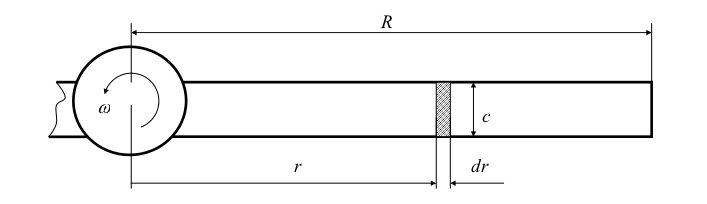
\includegraphics[width=0.45\textwidth]
  			{./pics_modelo_fisico/helice2.jpg}}
  \subfloat[Fuerzas aerodin\'amicas presentes en una h\'elice]{\label{fig:fuerza-helice} 
  		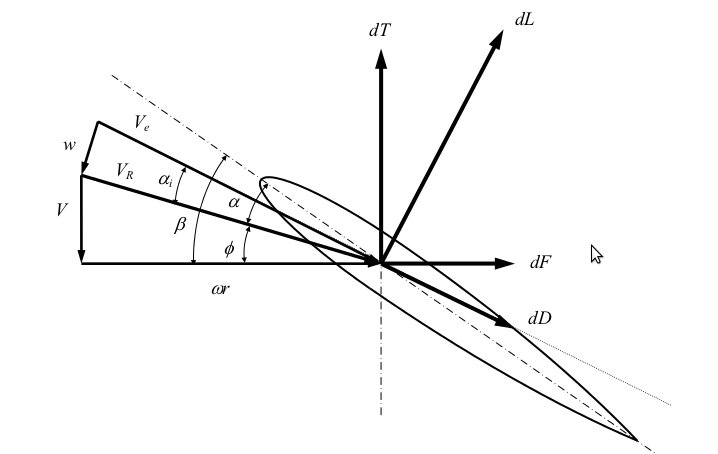
\includegraphics[width=0.45\textwidth]
  			{./pics_modelo_fisico/helice.jpg}}
  \caption{Vistas de una h\'elice y diagrama de fuerzas aerodin\'amicas presentes}
  \label{fig:helice}
\end{figure}

La \emph{Blade Element Theory}(BET) intenta explicar las fuerzas presentes en la h\'elice considerando en primer lugar las fuerzas en un elemento de \'area infinitesimal de la h\'elice. Una vez halladas estas fuerzas se integra sobre el total de la superficie obteniendo as\'i las fuerzas y momentos totales. Como se explica en \ref{bib:fuerzas-helices}, las fuerzas presentes sobre un elemento de \'area de la h\'elice son la fuerza de \emph{lift} y la fuerza de \emph{drag}, dichas fuerzas se encuentran representadas en la figura \ref{fig:helice} como $dL$ y $dD$ respectivamente. La forma que tienen dichas fuerzas es:

$$
dL=\frac{1}{2}\rho_A \omega_p^2 C_L c r^2dr$$\\

$$
dD=\frac{1}{2}\rho_A \omega_p^2 C_D c r^2dr
$$

Donde $\rho_A$ es la densidad del aire, $\omega_p$ la velocidad angular de la h\'elice, $r$ la distancia del elemento de h\'elice al eje de la h\'elice, c es la longitud promedio de la cuerda de la h\'elice \footnote{segmento imaginario que une el borde de ataque con el borde de fuga },$ C_L$ y $C_D$ son coeficientes adimensionados.

La fuerza infinitesimal de empuje ($dT$) puede escribirse en funci\'on de las fuerzas de \emph{lift} y de \emph{drag} de la siguiente forma:

$$dT=dL\cos\varphi_I-dD\sin\varphi$$

Realizando la aproximaci\'on que $\varphi$ es un \'angulo peque\~no y que la fuerza de \emph{lift} es al menos un orden mayor que la de \emph{drag} se puede afirmar que:

$$dT\approx dL
$$

El empuje por lo tanto puede calcularse como la integral de $dT$ respecto de $r$. Considerando que la h\'elice consta de dos hojas, se obtiene que:

\begin{equation}
\label{eq:fuerza}
T=\frac{1}{3}\rho_A C_L c R_P^3\omega_p^2
\end{equation}


Donde $R_P$ es el radio radio de la h\'elice. En todo momento tenemos dos fuerzas (una sobre cada hoja de la h\'elice) en direcci\'on vertical y hacia arriba. Si nos referimos a la configuraci\'on de la figura \ref{fig:fuerza-helice}, el momento de las fuerzas $dT$ es hacia la izquierda para la hoja considerada, sin embargo para la otra hoja este momento ser\'a hacia la derecha. Se puede concluir entonces que el torque neto que aporta esta fuerza en torno al eje de rotaci\'on de la h\'elice es nulo.\\   

Intentaremos ahora obtener la resultante de las fuerzas horizontales sobre la h\'elice y el torque de dichas fuerzas. Comenzaremos por analizar que sucede con las sumas de las fuerzas, para luego proceder a calcular el momento de las mismas. Consideremos ahora la fuerza $dF$ como la que se muestra en la figura \ref{fig:fuerza-helice}. Como se observa en la figura dicha fuerza es hacia la derecha. Si consideramos la fuerza horizontal sobre la otra hoja de la h\'elice, se obtiene una fuerza hacia la izquierda. Por lo tanto la suma de las fuerzas horizontales es nula. Sin embargo los momentos de las fuerzas en una y otra hoja de la h\'elice no se anulan, el momento que producen ambas es en la direcci\'on de $-\vec{k}_q$. Por lo tanto el momento total ser\'a la suma de los momentos infinitesimales en toda la superficie de una hoja de la h\'elice multiplicado por la cantidad de hojas, es decir 2. 

En primer lugar escribimos la fuerza horizontal como una composici\'on de la fuerza de \emph{lift} y la fuerza de \emph{drag}. 
$$dF=dD\cos\varphi+dL\sin\varphi \approx dD +dL\left(\frac{V}{\omega_p}\right)$$

En esta ecuaci\'on $V$ y $\omega_p r$ representan la velocidad del flujo de aire en las direcciones vertical y horizontal respectivamente. Operando se obtiene el momento total de la h\'elice en la direcci\'on entrante:

\begin{equation}
\label{eq:momento}
Q=\frac{1}{4}\rho_A c R_P^4(C_D+K)\omega_p^2
\end{equation}

 

En resumen, la teor\'ia BET nos permite afirmar que sobre cada h\'elice del cuadric\'optero que rota en sentido antihorario se aplicar\'a una fuerza en la direcci\'on $\vec{k_q}$ cuyo m\'odulo se expres\'o en la ecuaci\'on \ref{eq:fuerza} y un momento en la direcci\'on $-\vec{k_q}$ cuyo m\'odulo es lo expresado en la ecuaci\'on \ref{eq:momento}. Para una h\'elice rotando en sentido anti-horario se obtiene exactamente los mismos resultados excepto que el momento es en sentido opuesto.\\

Hasta aqu\'i sabemos que sucede las fuerzas y momentos aplicados sobre una h\'elice. Nos concentraremos ahora en estudiar como influyen estas fuerzas y momentos en el cuadric\'optero. Para lo que sigue continuaremos trabajando con las convenciones adoptadas en \ref{fig:quad}. 
 
A partir de lo estudiado anteriormente se deduce trivialmente que el empuje de las h\'elices puede expresarse en el sistema $S_q$ como:
$$
\sum_{i=1}^{i=4} \vec{T_i} =\sum_{i=1}^{i=4}T_i\left(\begin{array}{c}
0\\
0\\
1\\
\end{array} \right)
$$

Se determin\'o que las fuerzas de empuje no introducen un momento neto en el eje de las mismas. Sin embargo no debemos perder de vista que la segunda cardinal fue planteada en el centro de masa del sistema, por lo tanto respecto de dicho punto las fuerzas s\'i introducen un momento que puede calcularse como $M1=L\vec{x\prime} \times T1\vec{k_q}$ para el motor 1. $L$ es la distancia del centro de masa del cuadric\'optero al eje del motor 1. La expresi\'on del momento es an\'aloga para los restantes motores.

Debemos considerar adem\'as el momento obtenido para cada h\'elice en la direcci\'on $\vec{k_q}$. Cabe recordad que se dedujo que para h\'elices rotando en sentido anti- horario se tiene un momento positivo, mientras que para una h\'elice rotando en sentido horario el momento es negativo. Realizando estas consideraciones es posible afirmar que la suma total de los momentos es:

$$M_G^{ext} = \left(\begin{array}{c}
L(T2-T4)\\
L(T3-T1)\\
-Q_1+Q2-Q3+Q_4\\
\end{array} \right)$$

En base al estudio realizado se podr\'ian conocer dichas relaciones calculando los par\'ametros que dependen de la geometr\'ia de la h\'elice, sin embargo este estudio resulta tedioso y la mayor parte de los m\'etodos existentes para determinar dichos par\'ametros con buena precisi\'on son destructivos. Por lo tanto se opt\'o por obtener dichas respuestas en forma experimental. El proceso detallado puede consultarse en el anexo \ref{anexo motores}. En dichos experimentos se obtuvo que:

$$
T=3.5296\times 10^{-5}\omega^2-4.9293\times 10^{-4}\omega
$$\\$$Q= 3.4734\times 10^{-6}\omega^2-1.3205\times 10^{-4}\omega $$

Estos resultados parecen adecuados respecto de lo desarrollado te\'oricamente ya que ambas respuestas son cuadr\'aticas. 

\section{Modelo en variables de Estado}

Luego de realizados los estudios sobre la cinem\'atica y din\'amica del sistema y luego de comprender cabalmente las fuerzas y momentos involucrados se procede a construir el modelo en variables de estado.\\ 

Se debe aclarar que la elecci\'on realizada del vector de estados se debe exclusivamente a la conveniencia pr\'actica que se encuentra al trabajar con las variables expresadas en el sistema del cuadric\'optero. Esta conveniencia se ve reflejada en dos aspectos, en primer lugar las simplificaciones que introduce trabajar con estas variables en el marco de un desarrollo te\'orico de las ecuaciones que gobiernan al sistema, por otra parte, al disponer de sensores montados sobre el cuadric\'optero, los mismos medir\'an las velocidades angulares y lineales en el sistema $S_q$. Bajo esta elecci\'on parece razonable escoger el vector de estados de la siguiente manera:
$$X=\left\lbrace  x,y,z, \theta,\varphi,\psi, v_{q_z},v_{q_y},v_{q_z},\omega_{q_x},\omega_{q_y},\omega_{q_z} \right\rbrace$$

Las ecuaciones desarrolladas hasta ahora son las que gobiernan el comportamiento mecánico del sistema y son las que serán utilizadas para el desarrollo del simulador. Dichas ecuaciones dependen tanto de la velocidad angular de las hélices como de sus derivadas. Para realizar el control resulta m\'as sencillo poder trabajar sin dichas derivadas. La raz\'on es que las velocidades angulares y sus derivadas no son entradas independientes. Por lo tanto no se pueden imponer valores a unas sin considerar el comportamiento de las otras. En este sentido se realiza \'ultima aproximaci\'on. El t\'ermino de las derivadas de las velocidades angulares se encuentra presente exclusivamente en la ecuaci\'on \ref{eq:omegas}. Dicho t\'ermino se encuentra multiplicado por el momento de inercia de los motores. Considerando que la variaci\'on en la velocidad angular de los motores es inferior a la respuesta al escal\'on estudiada en \ref{chap:motores}, se puede despreciar el t\'ermino de las derivadas de las velocidades angulares respecto al t\'ermino asociado a los torques en la ecuaci\'on \ref{eq:omegas}.\\

Luego de realizada esta simplificaci\'on tenemos que la entrada est\'a compuesta por el vector:

$$u=\left\lbrace\omega_1, \omega_2, \omega_3, \omega_4\right\rbrace$$

El modelo en variables de estado es por lo tanto:

\begin{equation}
\boxed{\begin{aligned}&\dot{x}=v_{q_x} \cos \varphi \cos \theta + v_{q_y} ( \cos \theta \sin \varphi \sin \psi-\cos \varphi \sin \theta ) + v_{q_z}(\sin \psi \sin \theta + \cos \psi \cos \theta \sin \varphi)\\
&\dot{y}=v_{q_x} \cos \varphi \sin \theta + v_{q_y} (\cos \psi \cos \theta + \sin \theta \sin \varphi \sin \psi) + v_{q_z}( \cos \psi \sin \theta \sin \varphi-\cos \theta \sin \psi )\\
&\dot{z}= -v_{q_x} \sin \varphi  + v_{q_y} \cos \varphi \sin \psi  + v_{q_z}\cos \varphi \cos \psi\\
&\dot{\psi}=\omega_{q_x} + \omega_{q_z}\tan\varphi \cos\psi + \omega_{q_y}\tan\varphi \sin\psi\\
&\dot{\varphi}=\omega_{q_y}\cos \psi - \omega_{q_z}\sin\psi\\
&\dot{\theta}=\omega_{q_z} \frac{\cos\psi}{\cos\varphi}  + \omega_{q_y}\frac{\sin\psi}{\cos\varphi}\\
&\dot{v_{q_x}}=v_{q_y} \omega_{q_z} - v_{q_z} \omega_{q_y}+g\sin\varphi\\
&\dot{v_{q_y}}=v_{q_z} \omega_{q_x} - v_{q_x} \omega_{q_z}-g\cos\varphi\sin\psi\\
&\dot{v_{q_z}}=v_{q_x} \omega_{q_y} - v_{q_y} \omega_{q_x}-g\cos\varphi\cos\psi+\frac{1}{M}\sum_{i=1}^4T_i\\
&\dot{\omega_{q_x}}=\frac{\omega_{q_y}\omega_{q_z}(I_{yy}-I_{zz})+\omega_{q_y}I_{zz_m}(\omega_1-\omega_2+\omega_3-\omega_4)}{I_{xx}}+\frac{L(T_2-T_4)}{I_{xx}}\\
&\dot{\omega_{q_y}}=\frac{\omega_{q_x}\omega_{q_z}(-I_{xx}+I_{zz})+\omega_{q_x}I_{zz_m}(\omega_1-\omega_2+\omega_3-\omega_4)}{{I_{yy}}}+\frac{L(T_3-T_1)}{I_{yy}}\\
&\dot{\omega_{q_z}}=\frac{-Q_1+Q_2-Q_3+Q_4}{I_{zz}}\\
%\frac{-I_{zz_m}(\dot{w_1}-\dot{w_2}+\dot{w_3}-\dot{w_4})}{I_{zz}}+
\end{aligned}}
\label{eq:modelo}
\end{equation}









\end{document}

%Algunos layouts para poner im\'agnenes. Copien y peguen no
%m\'as. Hay figura com\'un, dos figuras en 1 onda fig 3a y 3b, wrapfigures y una matriz de figuras. Ta bueno, todas quedan lindas y andan bien.
%
%\begin{figure}[h!]
%	\centering
%	\includegraphics[width=0.75\textwidth]{./pics_modelo_fisico/		.eps}
%	\caption{		}
%	\label{fig:		}
%\end{figure}
%
%\begin{figure} [h!]
%  \centering
%  \subfloat[caption 1]{\label{fig:		}
%  		\includegraphics[width=0.45\textwidth]
%  			{./pics_modelo_fisico/		.eps}}
%  \subfloat[caption 2]{\label{fig:		} 
%  		\includegraphics[width=0.45\textwidth]
%  			{./pics_modelo_fisico/ 		.eps}}
%  \caption{Caption general}
%  \label{fig:	label general	}
%\end{figure}
%
%\begin{wrapfigure}{l}{0.6\textwidth}
%  \vspace{-20pt}
%  \begin{center}
%    \includegraphics[width=0.45\textwidth]
%    	{./pics_modelo_fisico/		.eps}
%  \end{center}
%  \vspace{-20pt}
%  \caption{		}
%  \label{ 		}
%  \vspace{-10pt}
%\end{wrapfigure}
%
%\begin{figure} [h!]
%  \begin{center}
%    \begin{tabular}{cc}
%      \resizebox{50mm}{!}
%      	{\includegraphics{./pics_modelo_fisico/ 	.eps}} &
%      \resizebox{50mm}{!}
%      	{\includegraphics{./pics_modelo_fisico/	.eps}} \\
%      \resizebox{50mm}{!}
%      	{\includegraphics{./pics_modelo_fisico/	.eps}} &
%      \resizebox{50mm}{!}
%      	{\includegraphics{./pics_modelo_fisico/	.eps}} \\
%    \end{tabular}
%    \caption{ 		}
%    \label{ 		}
%  \end{center}
%\end{figure}